\documentclass{standalone}
\usepackage{tikz}
\usetikzlibrary{patterns, positioning}

\begin{document}
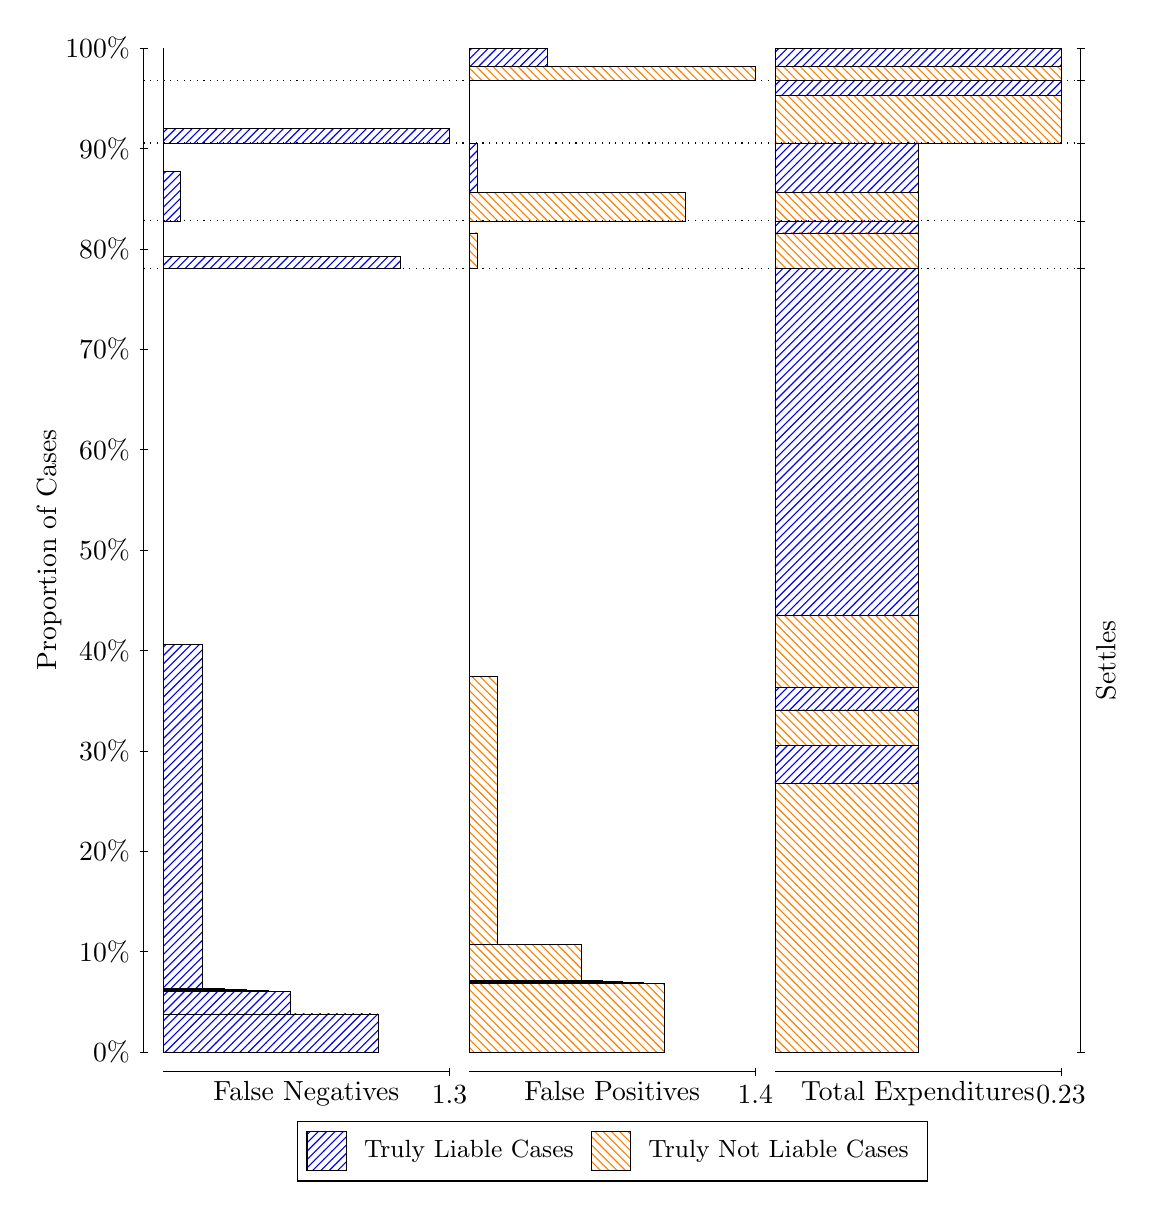
\begin{tikzpicture}
\draw[black, very thin] (1.5,1.75) -- (1.5,14.5);
\node[rotate=90, anchor=center] at (0.3, 8.125) {Proportion of Cases};
\draw[black, very thin] (1.45,1.75) -- (1.55,1.75);
\node[anchor=east] at (1.45, 1.75) {0\%};
\draw[black, very thin] (1.45,3.025) -- (1.55,3.025);
\node[anchor=east] at (1.45, 3.025) {10\%};
\draw[black, very thin] (1.45,4.3) -- (1.55,4.3);
\node[anchor=east] at (1.45, 4.3) {20\%};
\draw[black, very thin] (1.45,5.575) -- (1.55,5.575);
\node[anchor=east] at (1.45, 5.575) {30\%};
\draw[black, very thin] (1.45,6.85) -- (1.55,6.85);
\node[anchor=east] at (1.45, 6.85) {40\%};
\draw[black, very thin] (1.45,8.125) -- (1.55,8.125);
\node[anchor=east] at (1.45, 8.125) {50\%};
\draw[black, very thin] (1.45,9.4) -- (1.55,9.4);
\node[anchor=east] at (1.45, 9.4) {60\%};
\draw[black, very thin] (1.45,10.675) -- (1.55,10.675);
\node[anchor=east] at (1.45, 10.675) {70\%};
\draw[black, very thin] (1.45,11.95) -- (1.55,11.95);
\node[anchor=east] at (1.45, 11.95) {80\%};
\draw[black, very thin] (1.45,13.225) -- (1.55,13.225);
\node[anchor=east] at (1.45, 13.225) {90\%};
\draw[black, very thin] (1.45,14.5) -- (1.55,14.5);
\node[anchor=east] at (1.45, 14.5) {100\%};

\draw[black, very thin] (13.4,1.75) -- (13.4,14.5);
\draw[black, very thin] (13.35,1.75) -- (13.45,1.75);
\node[anchor=west] at (13.35, 1.75) {};
\draw[black, very thin] (13.35,11.7) -- (13.45,11.7);
\node[anchor=west] at (13.35, 11.7) {};
\draw[black, very thin] (13.35,12.306) -- (13.45,12.306);
\node[anchor=west] at (13.35, 12.306) {};
\draw[black, very thin] (13.35,13.294) -- (13.45,13.294);
\node[anchor=west] at (13.35, 13.294) {};
\draw[black, very thin] (13.35,14.087) -- (13.45,14.087);
\node[anchor=west] at (13.35, 14.087) {};
\draw[black, very thin] (13.35,14.5) -- (13.45,14.5);
\node[anchor=west] at (13.35, 14.5) {};

\draw[black, very thin, pattern color=blue, pattern=north east lines] (1.75,1.75) rectangle (4.475,2.2338);
\draw[black, very thin, pattern color=blue, pattern=north east lines] (1.75,2.2338) rectangle (3.3571,2.5211);
\draw[black, very thin, pattern color=blue, pattern=north east lines] (1.75,2.5211) rectangle (3.0776,2.5319);
\draw[black, very thin, pattern color=blue, pattern=north east lines] (1.75,2.5319) rectangle (2.7981,2.5429);
\draw[black, very thin, pattern color=blue, pattern=north east lines] (1.75,2.5429) rectangle (2.5186,2.5542);
\draw[black, very thin, pattern color=blue, pattern=north east lines] (1.75,2.5542) rectangle (2.2391,6.9275);
\draw[black, very thin, pattern color=orange, pattern=north west lines] (1.75,6.9275) rectangle (1.75,11.7);
\draw[black, very thin, pattern color=blue, pattern=north east lines] (1.75,11.7) rectangle (4.7545,11.855);
\draw[black, very thin, pattern color=orange, pattern=north west lines] (1.75,11.855) rectangle (1.75,12.306);
\draw[black, very thin, pattern color=blue, pattern=north east lines] (1.75,12.306) rectangle (1.9596,12.934);
\draw[black, very thin, pattern color=orange, pattern=north west lines] (1.75,12.934) rectangle (1.75,13.294);
\draw[black, very thin, pattern color=blue, pattern=north east lines] (1.75,13.294) rectangle (5.3833,13.479);
\draw[black, very thin, pattern color=orange, pattern=north west lines] (1.75,13.479) rectangle (1.75,14.087);
\draw[black, very thin, pattern color=orange, pattern=north west lines] (1.75,14.087) rectangle (1.75,14.27);
\draw[black, very thin, pattern color=blue, pattern=north east lines] (1.75,14.27) rectangle (1.75,14.5);
\draw[black, very thin, pattern color=orange, pattern=north west lines] (5.6333,1.75) rectangle (8.1106,2.6221);
\draw[black, very thin, pattern color=orange, pattern=north west lines] (5.6333,2.6221) rectangle (7.8464,2.6354);
\draw[black, very thin, pattern color=orange, pattern=north west lines] (5.6333,2.6354) rectangle (7.5821,2.6485);
\draw[black, very thin, pattern color=orange, pattern=north west lines] (5.6333,2.6485) rectangle (7.3179,2.6612);
\draw[black, very thin, pattern color=orange, pattern=north west lines] (5.6333,2.6612) rectangle (7.0536,3.1124);
\draw[black, very thin, pattern color=orange, pattern=north west lines] (5.6333,3.1124) rectangle (5.9967,6.5224);
\draw[black, very thin, pattern color=blue, pattern=north east lines] (5.6333,6.5224) rectangle (5.6333,11.7);
\draw[black, very thin, pattern color=orange, pattern=north west lines] (5.6333,11.7) rectangle (5.7324,12.151);
\draw[black, very thin, pattern color=blue, pattern=north east lines] (5.6333,12.151) rectangle (5.6333,12.306);
\draw[black, very thin, pattern color=orange, pattern=north west lines] (5.6333,12.306) rectangle (8.3748,12.666);
\draw[black, very thin, pattern color=blue, pattern=north east lines] (5.6333,12.666) rectangle (5.7324,13.294);
\draw[black, very thin, pattern color=orange, pattern=north west lines] (5.6333,13.294) rectangle (5.6333,13.903);
\draw[black, very thin, pattern color=blue, pattern=north east lines] (5.6333,13.903) rectangle (5.6333,14.087);
\draw[black, very thin, pattern color=orange, pattern=north west lines] (5.6333,14.087) rectangle (9.2667,14.27);
\draw[black, very thin, pattern color=blue, pattern=north east lines] (5.6333,14.27) rectangle (6.6242,14.5);
\draw[black, very thin, pattern color=orange, pattern=north west lines] (9.5167,1.75) rectangle (11.333,5.16);
\draw[black, very thin, pattern color=blue, pattern=north east lines] (9.5167,5.16) rectangle (11.333,5.6438);
\draw[black, very thin, pattern color=orange, pattern=north west lines] (9.5167,5.6438) rectangle (11.333,6.095);
\draw[black, very thin, pattern color=blue, pattern=north east lines] (9.5167,6.095) rectangle (11.333,6.3823);
\draw[black, very thin, pattern color=orange, pattern=north west lines] (9.5167,6.3823) rectangle (11.333,7.2935);
\draw[black, very thin, pattern color=blue, pattern=north east lines] (9.5167,7.2935) rectangle (11.333,11.7);
\draw[black, very thin, pattern color=orange, pattern=north west lines] (9.5167,11.7) rectangle (11.333,12.151);
\draw[black, very thin, pattern color=blue, pattern=north east lines] (9.5167,12.151) rectangle (11.333,12.306);
\draw[black, very thin, pattern color=orange, pattern=north west lines] (9.5167,12.306) rectangle (11.333,12.666);
\draw[black, very thin, pattern color=blue, pattern=north east lines] (9.5167,12.666) rectangle (11.333,13.294);
\draw[black, very thin, pattern color=orange, pattern=north west lines] (9.5167,13.294) rectangle (13.15,13.903);
\draw[black, very thin, pattern color=blue, pattern=north east lines] (9.5167,13.903) rectangle (13.15,14.087);
\draw[black, very thin, pattern color=orange, pattern=north west lines] (9.5167,14.087) rectangle (13.15,14.27);
\draw[black, very thin, pattern color=blue, pattern=north east lines] (9.5167,14.27) rectangle (13.15,14.5);
\draw[black, dotted] (1.5,11.7) -- (13.4,11.7);
\draw[black, dotted] (1.5,12.306) -- (13.4,12.306);
\draw[black, dotted] (1.5,13.294) -- (13.4,13.294);
\draw[black, dotted] (1.5,14.087) -- (13.4,14.087);
\draw[black, very thin] (1.75,1.5) -- (5.3833,1.5);
\node[anchor=north] at (3.5667, 1.5) {False Negatives};
\draw[black, very thin] (5.3833,1.45) -- (5.3833,1.55);
\node[anchor=north] at (5.3833, 1.45) {1.3};

\draw[black, very thin] (5.6333,1.5) -- (9.2667,1.5);
\node[anchor=north] at (7.45, 1.5) {False Positives};
\draw[black, very thin] (9.2667,1.45) -- (9.2667,1.55);
\node[anchor=north] at (9.2667, 1.45) {1.4};

\draw[black, very thin] (9.5167,1.5) -- (13.15,1.5);
\node[anchor=north] at (11.333, 1.5) {Total Expenditures};
\draw[black, very thin] (13.15,1.45) -- (13.15,1.55);
\node[anchor=north] at (13.15, 1.45) {0.23};

\node[black, centered, rotate=90] at (13.72, 6.725) {Settles};





\draw (7.449999999999999,1.5) node[draw=none] (baseCoordinate) {};
\begin{scope}[align=center]
        \matrix[scale=0.5, draw=black, below=0.5cm of baseCoordinate, nodes={draw}, column sep=0.1cm]{
            \node[rectangle, draw, minimum width=0.5cm, minimum height=0.5cm, pattern=north east lines, pattern color=blue] {}; &
            \node[draw=none, font=\small] (B) {Truly Liable Cases}; &
            \node[rectangle, draw, minimum width=0.5cm, minimum height=0.5cm, pattern=north west lines, pattern color=orange] {}; &
            \node[draw=none, font=\small] (B) {Truly Not Liable Cases}; \\
            };
\end{scope}

\end{tikzpicture}
\end{document}